% ============================================================
\chapter{Descente de Gradient et Variantes}
\label{ch:gradient}
% ============================================================

\section{Introduction}

Augustin-Louis Cauchy, en 1847, propose une id\'ee d'une simplicit\'e d\'esarmante~: pour minimiser une fonction, il suffit de suivre la direction oppos\'ee au gradient. Comme une bille qui roule sur une surface, on descend la pente la plus raide, pas apr\`es pas, jusqu'\`a atteindre le fond de la vall\'ee. Cette m\'ethode, la \emph{descente de gradient}, est rest\'ee longtemps un outil th\'eorique. Mais l'explosion de l'apprentissage automatique au XXI\ieme{} si\`ecle l'a propuls\'ee au rang d'algorithme le plus ex\'ecut\'e au monde~: chaque fois qu'un r\'eseau de neurones apprend, c'est une variante de la descente de gradient qui ajuste ses milliards de param\`etres. Les questions fondamentales --- quel pas choisir~? comment acc\'el\'erer la convergence~? que faire quand le gradient est trop co\^uteux \`a calculer exactement~? --- ont conduit aux m\'ethodes de Nesterov, d'Adam, et au gradient stochastique, qui forment aujourd'hui la bo\^ite \`a outils incontournable de l'optimisation moderne.

\section{Descente de gradient \`a pas fixe}

\begin{algorithme}[title=\textbf{Descente de gradient}]
\begin{enumerate}
    \item Choisir $x_0 \in \R^n$, pas $\alpha > 0$.
    \item Pour $k = 0, 1, 2, \ldots$~:
    \[
        x_{k+1} = x_k - \alpha \nabla f(x_k).
    \]
    \item Arr\^eter quand $\norm{\nabla f(x_k)} < \varepsilon$.
\end{enumerate}
\end{algorithme}

\begin{intuition}
\`A chaque it\'eration, on se d\'eplace dans la direction oppos\'ee au gradient
(direction de plus forte descente locale) avec un pas $\alpha$. Le gradient pointe
dans la direction de plus forte mont\'ee, donc $-\nabla f(x_k)$ est la direction
de plus forte descente.
\end{intuition}

\section{Analyse de convergence --- fonctions $L$-lisses}

\begin{theoreme}[Convergence pour fonctions convexes $L$-lisses]
\label{thm:conv_lisse}
Soit $f$ convexe et $L$-lisse. Avec le pas $\alpha = 1/L$~:
\[
    f(x_k) - f^* \leq \frac{L\norm{x_0 - x^*}^2}{2k}.
\]
Le taux de convergence est $O(1/k)$.
\end{theoreme}

\begin{proof}
Par la $L$-lissit\'e, pour $\alpha = 1/L$~:
\[
    f(x_{k+1}) \leq f(x_k) + \inner{\nabla f(x_k)}{x_{k+1} - x_k} + \frac{L}{2}\norm{x_{k+1} - x_k}^2.
\]
Avec $x_{k+1} - x_k = -\frac{1}{L}\nabla f(x_k)$~:
\[
    f(x_{k+1}) \leq f(x_k) - \frac{1}{2L}\norm{\nabla f(x_k)}^2.
\]

Par la condition du premier ordre~: $f(x_k) - f^* \leq \inner{\nabla f(x_k)}{x_k - x^*}
\leq \norm{\nabla f(x_k)}\norm{x_k - x^*}$, donc~:
\[
    \norm{\nabla f(x_k)}^2 \geq \frac{(f(x_k) - f^*)^2}{\norm{x_k - x^*}^2}.
\]

De plus, $\norm{x_{k+1} - x^*}^2 = \norm{x_k - x^*}^2 - \frac{2}{L}\inner{\nabla f(x_k)}{x_k - x^*} + \frac{1}{L^2}\norm{\nabla f(x_k)}^2$.

En posant $\delta_k = f(x_k) - f^*$ et $R_k = \norm{x_k - x^*}^2$~:
\[
    \delta_{k+1} \leq \delta_k - \frac{1}{2L}\norm{\nabla f(x_k)}^2, \quad
    R_{k+1} \leq R_k - \frac{2}{L}\delta_k + \frac{1}{L^2}\norm{\nabla f(x_k)}^2.
\]

En sommant la d\'ecroissance suffisante~:
$\sum_{i=0}^{k-1} \frac{1}{2L}\norm{\nabla f(x_i)}^2 \leq \delta_0$, et par
un argument t\'elescopique sur $R_k$~:
\[
    \sum_{i=0}^{k-1} \delta_i \leq \frac{L}{2}R_0.
\]
Comme $\delta_k$ est d\'ecroissante~: $k\delta_k \leq \sum_{i=0}^{k-1}\delta_i \leq \frac{L}{2}R_0$.
\end{proof}

\section{Convergence pour fonctions fortement convexes}

\begin{theoreme}[Convergence lin\'eaire]
\label{thm:conv_forte}
Soit $f$ $m$-fortement convexe et $L$-lisse. Avec $\alpha = 1/L$~:
\[
    f(x_k) - f^* \leq \left(1 - \frac{m}{L}\right)^k (f(x_0) - f^*).
\]
Le taux est lin\'eaire (convergence g\'eom\'etrique) avec facteur $1 - 1/\kappa$
o\`u $\kappa = L/m$ est le nombre de conditionnement.
\end{theoreme}

\begin{proof}
Par la $L$-lissit\'e et le pas $\alpha = 1/L$~:
$f(x_{k+1}) \leq f(x_k) - \frac{1}{2L}\norm{\nabla f(x_k)}^2$.

Par la forte convexit\'e~: $\norm{\nabla f(x_k)}^2 \geq 2m(f(x_k) - f^*)$
(in\'egalit\'e de Polyak--\L{}ojasiewicz). Donc~:
\[
    f(x_{k+1}) - f^* \leq (f(x_k) - f^*) - \frac{m}{L}(f(x_k) - f^*)
    = \left(1 - \frac{m}{L}\right)(f(x_k) - f^*).
\]
\end{proof}

\begin{formules}[title=\textbf{R\'esum\'e des taux de convergence}]
\begin{center}
\renewcommand{\arraystretch}{1.3}
\begin{tabular}{lcc}
\toprule
\textbf{Hypoth\`ese} & \textbf{Taux} & \textbf{Complexit\'e pour $\varepsilon$} \\
\midrule
Convexe, $L$-lisse & $O(1/k)$ & $O(L/\varepsilon)$ \\
$m$-fort. convexe, $L$-lisse & $O((1-m/L)^k)$ & $O(\kappa\log(1/\varepsilon))$ \\
Convexe, non lisse & $O(1/\sqrt{k})$ & $O(1/\varepsilon^2)$ \\
\bottomrule
\end{tabular}
\end{center}
\end{formules}

\section{Recherche de pas (line search)}

\begin{definition}[Condition d'Armijo (backtracking)]
Choisir $\alpha_k$ comme le plus grand $\alpha = \beta^j \hat{\alpha}$ ($j = 0,1,\ldots$)
satisfaisant~:
\[
    f(x_k - \alpha\nabla f(x_k)) \leq f(x_k) - c\alpha\norm{\nabla f(x_k)}^2,
\]
avec $c \in (0, 1/2)$ et $\beta \in (0,1)$.
\end{definition}

\begin{proposition}
La descente de gradient avec backtracking d'Armijo conserve les m\^emes taux de
convergence $O(1/k)$ et $O((1-m/L)^k)$ (avec des constantes diff\'erentes).
\end{proposition}

\section{Gradient acc\'el\'er\'e de Nesterov}

\begin{algorithme}[title=\textbf{Gradient acc\'el\'er\'e de Nesterov (NAG)}]
\begin{enumerate}
    \item Initialiser $x_0 = y_0 \in \R^n$.
    \item Pour $k = 0, 1, 2, \ldots$~:
    \begin{align*}
        x_{k+1} &= y_k - \frac{1}{L}\nabla f(y_k), \\
        y_{k+1} &= x_{k+1} + \frac{k}{k+3}(x_{k+1} - x_k).
    \end{align*}
\end{enumerate}
\end{algorithme}

\begin{theoreme}[Convergence de Nesterov]
\label{thm:nesterov}
Soit $f$ convexe et $L$-lisse. L'algorithme de Nesterov satisfait~:
\[
    f(x_k) - f^* \leq \frac{2L\norm{x_0 - x^*}^2}{(k+1)^2}.
\]
Le taux $O(1/k^2)$ est optimal parmi les m\'ethodes du premier ordre
(borne inf\'erieure de Nemirovski--Yudin).
\end{theoreme}

\begin{attention}[title=\textbf{Optimalit\'e du taux $O(1/k^2)$}]
Nemirovski et Yudin (1983) ont montr\'e qu'aucune m\'ethode du premier ordre
(n'utilisant que les valeurs de $f$ et $\nabla f$) ne peut converger plus vite que
$O(1/k^2)$ pour la classe des fonctions convexes $L$-lisses. L'acc\'el\'eration de
Nesterov atteint cette borne~: elle est \emph{optimale}.
\end{attention}

\section{Gradient conjugu\'e}

\begin{algorithme}[title=\textbf{Gradient conjugu\'e non lin\'eaire (Fletcher--Reeves)}]
\begin{enumerate}
    \item $d_0 = -\nabla f(x_0)$.
    \item Pour $k = 0, 1, 2, \ldots$~:
    \begin{enumerate}
        \item $\alpha_k = \argmin_{\alpha > 0} f(x_k + \alpha d_k)$.
        \item $x_{k+1} = x_k + \alpha_k d_k$.
        \item $\beta_{k+1} = \frac{\norm{\nabla f(x_{k+1})}^2}{\norm{\nabla f(x_k)}^2}$.
        \item $d_{k+1} = -\nabla f(x_{k+1}) + \beta_{k+1} d_k$.
    \end{enumerate}
\end{enumerate}
\end{algorithme}

\begin{remarque}
Pour une fonction quadratique $f(x) = \frac{1}{2}x^TAx - b^Tx$ avec $A \succ 0$,
le gradient conjugu\'e converge en au plus $n$ it\'erations (convergence finie).
\end{remarque}

\section{Gradient stochastique (SGD)}

\begin{algorithme}[title=\textbf{Descente de gradient stochastique}]
Pour $f(x) = \frac{1}{N}\sum_{i=1}^N f_i(x)$~:
\begin{enumerate}
    \item Pour $k = 0, 1, 2, \ldots$~:
    \begin{enumerate}
        \item Tirer $i_k$ uniform\'ement dans $\{1, \ldots, N\}$.
        \item $x_{k+1} = x_k - \alpha_k \nabla f_{i_k}(x_k)$.
    \end{enumerate}
\end{enumerate}
\end{algorithme}

\begin{theoreme}[Convergence du SGD]
Pour $f$ convexe, $L$-lisse, avec $\mathbb{E}[\norm{\nabla f_i(x) - \nabla f(x)}^2] \leq \sigma^2$
et $\alpha_k = c/\sqrt{k}$~:
\[
    \mathbb{E}[f(\bar{x}_k)] - f^* = O\left(\frac{1}{\sqrt{k}}\right),
\]
o\`u $\bar{x}_k = \frac{1}{k}\sum_{i=1}^k x_i$.
Pour $f$ $m$-fortement convexe avec $\alpha_k = 1/(mk)$~:
\[
    \mathbb{E}[f(\bar{x}_k)] - f^* = O\left(\frac{1}{k}\right).
\]
\end{theoreme}

\section{Variantes modernes du SGD}

\begin{algorithme}[title=\textbf{Adam (Kingma \& Ba, 2015)}]
\begin{enumerate}
    \item Param\`etres~: $\beta_1 = 0.9$, $\beta_2 = 0.999$, $\varepsilon = 10^{-8}$, $\alpha$.
    \item $m_0 = 0$, $v_0 = 0$.
    \item Pour $k = 1, 2, \ldots$~:
    \begin{align*}
        g_k &= \nabla f_{i_k}(x_k), \\
        m_k &= \beta_1 m_{k-1} + (1-\beta_1) g_k, \\
        v_k &= \beta_2 v_{k-1} + (1-\beta_2) g_k^2, \\
        \hat{m}_k &= m_k / (1 - \beta_1^k), \\
        \hat{v}_k &= v_k / (1 - \beta_2^k), \\
        x_{k+1} &= x_k - \alpha \hat{m}_k / (\sqrt{\hat{v}_k} + \varepsilon).
    \end{align*}
\end{enumerate}
\end{algorithme}

\section{Interpr\'etation g\'eom\'etrique}

\begin{center}
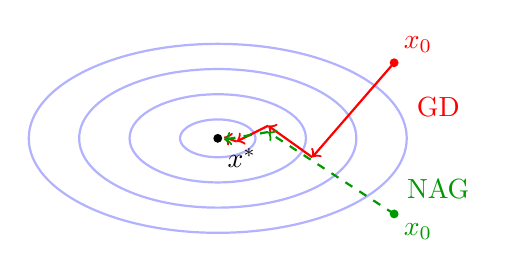
\begin{tikzpicture}[scale=0.8]
    % Contour lines of quadratic
    \draw[blue!30, thick] (0,0) ellipse (3 and 1.5);
    \draw[blue!30, thick] (0,0) ellipse (2.2 and 1.1);
    \draw[blue!30, thick] (0,0) ellipse (1.4 and 0.7);
    \draw[blue!30, thick] (0,0) ellipse (0.6 and 0.3);

    % Gradient descent path
    \draw[->, thick, red] (2.8, 1.2) -- (1.5, -0.3);
    \draw[->, thick, red] (1.5, -0.3) -- (0.8, 0.2);
    \draw[->, thick, red] (0.8, 0.2) -- (0.3, -0.05);
    \draw[->, thick, red] (0.3, -0.05) -- (0.1, 0.02);

    \fill[red] (2.8, 1.2) circle (2pt) node[above right] {$x_0$};
    \fill[black] (0,0) circle (2pt) node[below right] {$x^*$};

    % Nesterov path
    \draw[->, thick, green!60!black, dashed] (2.8, -1.2) -- (0.8, 0.1);
    \draw[->, thick, green!60!black, dashed] (0.8, 0.1) -- (0.1, -0.02);

    \fill[green!60!black] (2.8, -1.2) circle (2pt) node[below right] {$x_0$};

    \node[red] at (3.5, 0.5) {GD};
    \node[green!60!black] at (3.5, -0.8) {NAG};
\end{tikzpicture}
\end{center}

\section{Impl\'ementation Python}

\begin{codeblock}[title=\textbf{Comparaison GD, Nesterov et SGD}]
\begin{minted}{python}
import numpy as np
import matplotlib.pyplot as plt

def gradient_descent(f, grad_f, x0, L, n_iter):
    x = x0.copy()
    history = [f(x)]
    for k in range(n_iter):
        x = x - (1/L) * grad_f(x)
        history.append(f(x))
    return x, history

def nesterov_accelerated(f, grad_f, x0, L, n_iter):
    x = x0.copy()
    y = x0.copy()
    history = [f(x)]
    for k in range(n_iter):
        x_new = y - (1/L) * grad_f(y)
        y = x_new + (k / (k + 3)) * (x_new - x)
        x = x_new
        history.append(f(x))
    return x, history

# Quadratique mal conditionnee
np.random.seed(42)
n = 50
eigvals = np.logspace(-2, 2, n)  # kappa = 10000
Q_diag = eigvals
b = np.random.randn(n)

f = lambda x: 0.5 * np.sum(Q_diag * x**2) - np.sum(b * x)
grad_f = lambda x: Q_diag * x - b
L = np.max(Q_diag)
f_star = -0.5 * np.sum(b**2 / Q_diag)

x0 = np.zeros(n)
_, hist_gd = gradient_descent(f, grad_f, x0, L, 500)
_, hist_nag = nesterov_accelerated(f, grad_f, x0, L, 500)

plt.semilogy(np.array(hist_gd) - f_star, label='GD')
plt.semilogy(np.array(hist_nag) - f_star, label='Nesterov')
plt.xlabel('Iteration k')
plt.ylabel('$f(x_k) - f^*$')
plt.legend()
plt.title('GD vs Nesterov (kappa=10000)')
plt.grid(True, alpha=0.3)
plt.savefig('gd_vs_nesterov.pdf')
\end{minted}
\end{codeblock}

\section{Exercices}

\begin{exercice}[$\star$]
Montrer que pour $f(x) = \frac{1}{2}\norm{Ax-b}^2$, le gradient est $\nabla f(x) = A^T(Ax-b)$
et la constante de lissit\'e est $L = \norm{A^TA}$.
\end{exercice}

\begin{exercice}[$\star\star$]
D\'emontrer l'in\'egalit\'e de Polyak--\L{}ojasiewicz~: si $f$ est $m$-fortement
convexe, alors $\norm{\nabla f(x)}^2 \geq 2m(f(x) - f^*)$.
\end{exercice}

\begin{exercice}[$\star\star$]
Impl\'ementer le backtracking d'Armijo et comparer avec le pas fixe $1/L$ sur
un probl\`eme de r\'egression logistique.
\end{exercice}

\begin{exercice}[$\star\star$]
Montrer que le gradient conjugu\'e converge en au plus $n$ it\'erations pour une
quadratique en dimension $n$.
\end{exercice}

\begin{exercice}[$\star\star\star$]
D\'emontrer la borne de convergence $O(1/k^2)$ du gradient acc\'el\'er\'e de
Nesterov en utilisant une fonction de Lyapunov.
\end{exercice}

\begin{exercice}[$\star\star\star$]
Montrer la borne inf\'erieure de Nemirovski--Yudin~: il existe une fonction convexe
$L$-lisse telle que toute m\'ethode du premier ordre satisfait
$f(x_k) - f^* \geq \frac{cL\norm{x_0-x^*}^2}{k^2}$ pour $k \leq (n-1)/2$.
\end{exercice}
